\chapter{Design of the Envoy File System}

This chapter examines the storage needs of service clusters and how they can be accommodated. Service clusters place specific demands on the storage system to efficiently support the deployment and management of untrusted services, but they also present helpful properties that can simplify the job. In addition to detailing these constraints, this chapter describes Envoy, a file system designed for this environment.

\section{Design goals and principles}

\subsection{Things that a service cluster calls for}
\begin{itemize}
\item exploit admin domain for simple security and fault model
\item expect lots of redundancy in disk images; aggregate cache
\item support mobile VMs
\item support rapid deployment of services with lightweight file system forks
\item use cheap commodity disks
\item snapshots
\item isolate services from each other, but allow cooperative groups
\end{itemize}

\subsection{Desirable properties that the envoy model achieves}
\begin{itemize}
\item distribute only when there's a reason; favor centralization when practical
\item perfectly consistent persistent caching
\item local impact---heavy users bear most of the load, non-users none of it
\item serve from local machine cache when uncontended, NFS-like when shared: requests never require topology changes
\item in steady state, coordination based on actual contention, not potential contention
\item simple security model that maps well to familiar Unix semantics
\item private images act like local images, shared images scale gracefully
\end{itemize}

\section{Using Envoy}

\subsection{Basic environment and assumptions}



It's a cluster, dom0 is trusted, it's all managed together, expect users to start from standard installs

\subsection{Use and administration}

This section presents the administrative interface to Envoy, which is designed as a series of special file operations and conventions.

All services share a single cluster-wide namespace tree with a common root. Mounting the root of the entire tree requires special priviledges, normally reserved for the administrative tools managing the file system. The top levels of the hierachy respond normally to standard file operations, with a few notable exceptions described here.

A few file names are given special significance and their use is restricted. The name \current is reserved for use as the root of a client file system, positive integers are reserved as the read-only roots of snapshots (in ascending order) of the tree rooted at \current in the same directory, and a symbolic link names \snapshot is created and protected by the system to link to the most recently-created snapshot in the same directory. In addition, a normal file named \password can exist to store credentials for clients accessing descendents of the containing directory.

The namespace is conceptually divided between the administrative levels and the client levels. The client levels include anything that is a descendent of a directory named \current or one of its snapshots (named as positive integers). Any path that does not pass through one of these points is considered part of the administrative namespace and is subject to the restrictions and special semantics described in this section.

To create a new file system root, a user or management tool creates any desired layers of files and directories within the administrative area, ending with a directory called \current. Services can then mount \current or any of its descendent directories. A client mount request specifies the desired root pathname along with the username attempting the mount and any credentials required to validate the request. The server checks these credentials against any files called \password that it encounters in administrative directories passed through before arriving at \current, with those further down the hierarchy overriding those encountered earlier.

In addition to end-user mounts, this system of password files applies to the administrative file areas as well. If given suitable credentials, a service can attach to the namespace in an administrative directory to create and manage its own file system trees and credential files, creating a hierachy for management roles as well as file storage. Controlling access to any directory requires credentials to mount its parent, along with standard file permissions within the parent directory to manipulate the credential file. Envoy does not map user and group names to numeric IDs, so any clients that can agree on usernames and credentials can share access to a file system.

The \current directory---in addition to marking the transition from administrative to client directories--- can have its snapshot taken. When the server receives a request to create a symbolic link with a positive integer as its name and \current as its target, it checks to make sure that the integer is correct for the next snapshot (either \texttt{1} or the number linked to by \snapshot plus one). If so, it takes a snapshot of \current, makes it accessible using the requested name (accessible as a directory, not a symbolic link), and creates or updates \snapshot to link to the newly created snapshot. Any request with the wrong target or the wrong number is rejected.

Snapshots are always given positive integers as names (and cannot be renamed), but this is not always convenient for use. It may be useful to name a particular snapshot with a more meaningful name using a symbolic link. Symbolic links are normally considered opaque by the server and cannot be used in any mount or directory-change requests, so to make accessing named snapshots more convenient the server silently dereferences symbolic links that refer to snapshots in the same directory.

Snapshots also serve another special purpose: they can be used as the root for a file system fork operation. Just as the \current directory diverges from its most recent snapshot using copy-on-write semantics, new \current roots in other administrative directories can use an existing snapshot as a starting point. A request to create a symbolic link called \current that refers to the fully-qualified pathname of a snapshot (again, links to a snapshot within the same directory are dereferenced, but others are not) is treated as a fork operation using the given snapshot as the starting point for a new root file system. The newly forked file system is subject to the same rules as those created with \texttt{mkdir}, and respects the credentials local to its creation site, not those of the snapshot from which it diverges. For this reason, fork operations require sufficient credentials at both locations.

\section{Architecture}

Services access Envoy using a client-server network file system interface. Each physical machine in the service cluster runs an administrative virtual machine that manages the storage processes for all services on that machine. The services on this VM partition the local disk between a constribution to the shared storage pool and the local persistent cache as well as providing a standard interface allowing other hosts on the machine to access the file system. \prettyref{fig:single-machine} illustrates a typical machine.

\begin{figure}[tp]
\centering
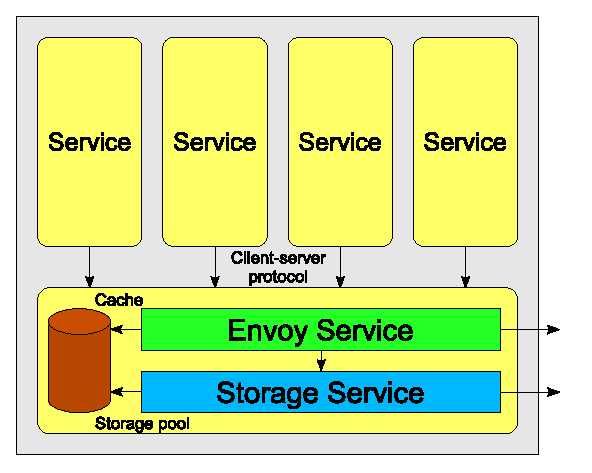
\includegraphics{figures/single-machine}
\caption{Each physical machine has a single administrative VM that hosts the Envoy services. This VM exports a network file system protocol to other service VMs running on the same machine.}
\label{fig:single-machine}
\end{figure}

The file system management processes join a cluster-wide service that is comprised of two primary layers, as illustrated in \prettyref{fig:layers}. Storage is managed by the lower level, which allows a small set of basic file operations on objects. All operations are stateless and the storage service makes no attempt to prevent or manage concurrent requests or to enforce any kind of security policy. Objects are extents of bytes with a small set of attributes.

On top of the storage service is the Envoy layer, which builds a hierarchical file system out of objects, coordinates access to files, provides authentication and access control services, manages caching, and exports a standard network file system interface for services to access.

\begin{figure}[tp]
\centering
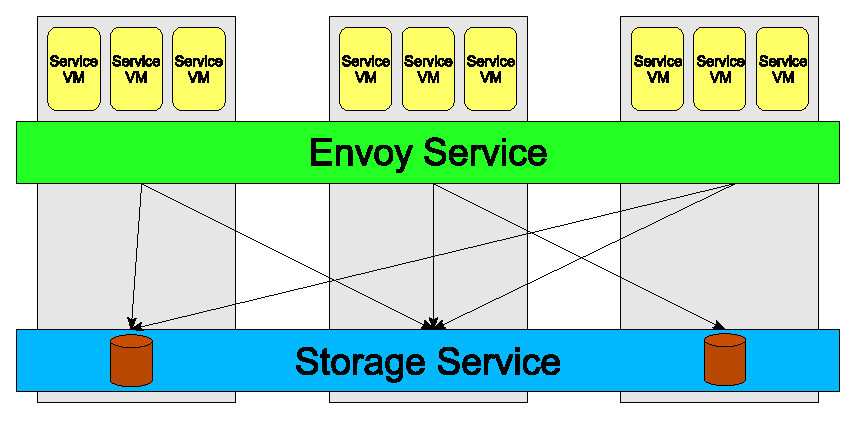
\includegraphics{figures/layers}
\caption{The Envoy services coordinate access to provide a single, coherent view of the distributed file system. It relies on the storage service, which provides a repository of objects referenced by unique identifiers.}
\label{fig:layers}
\end{figure}

In the remainder of this section I detail the functionality and requirements of these systems and consider the tradeoffs of various design decisions.

\subsection{Distribution}

\prettyref{fig:client-server} depicts a commonly-used storage arrangement using a series of dedicated file servers to handle the needs of many clients. This architecture is successfully used in many settings and, despite alternatives developed over the years, is still the dominant storage model in practical use.

\begin{figure}[tp]
\centering
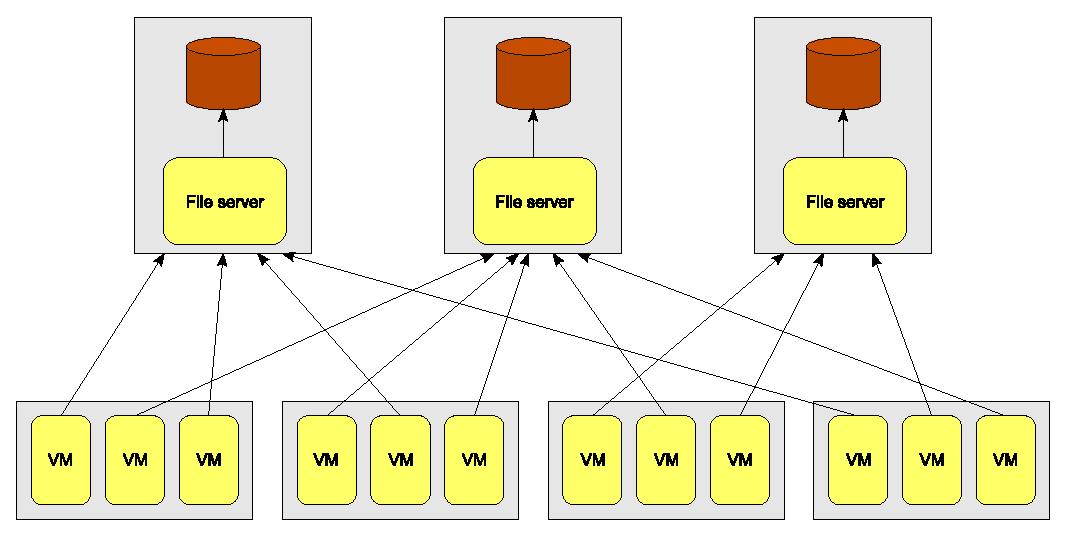
\includegraphics[width=100mm]{figures/client-server}
\caption{A popular storage solution for groups of clients involves a series of dedicated servers. Content on the servers is carefully managed to distributed storage demand and transaction load between the servers.}
\label{fig:client-server}
\end{figure}

The client-server model has obvious flaws when applied to clusters with many transient clients. Data placement decisions must balance space requirements and expected access rates in order to avoid overloading a particular server. Rebalancing---a disruptive and time consuming job---may be necessary in response to added clients, added servers, added disks, variations in client workload, and accumulation of data over time.

With the service cluster model, the problem is made even worse. To make efficient use of increasingly powerful hardware, each physical machine may host many services, each of which requires a boot image as well as access to the data relevant to its intended task. Single-purpose services may also be short lived or vary by time of data, making manual balancing impractical.

The client-server model has not endured as long as it has simply for lack of alternatives, however. It has many strengths that can inform the design of a more distributed architecture. With a single server managing shared data, concurrent access can be managed simply through explicit leases and cache invalidation, centralized caching with synchronous access, or through a lock manager. Whatever the mechanism for resolving conflicts, a centralized server is ideally suited to detecting and responding to concurrent requests because it is the point on the access graph at which all requests converge. The consistency of data that has reached the server is as good as its backing store.

The simplicity of a server is also a virtue. A failstop model for reliability can generally be assumed, backups are relatively straightforward, the server is typically dedicated to a single task or is shared with other trusted services, and the semantics are simple to define in terms of client behavior%
\footnote{NFS versions 2 and 3 have notoriously complicated consistency semantics, but this is almost entirely due to client policies. NFS server semantics are straightforward.}.

The chief faults of a centralized system are the introduction of a single point of failure and the inability to scale beyond the network and disk bandwidth that can be hosted by a single server. While these limits are unacceptable at large scales, they are quite reasonable for small groups of clients.

For clients that are sharing data, it is difficult to improve on a centralized server. For sufficiently overlapping data sets, any consistent model will degrade to something resembling a server during periods of contention because all interested clients will have to synchronize their access to the contended bits. A single arbitrator will ultimately oversee each bit of data, whether it is a traditional server, a lease-holding client, or a quorum of cooperating peers.

Sharing cache space is also a benefit of consolidated control of shared data. As the performance gap between disk access and memory access continues to grow, efficient use available cache space becomes increasingly important. Once again, a single centralized cache fails the scalability requirement, but a shared cache for a smaller set of clients with overlapping data needs provides attractive properties. Accessing a cache across a high-speed network is faster than accessing a local disk \cite{dahlin94b}, so in a cluster setting, organizing the aggregate cache around shared access patterns is more valuable than organizing it to localize access. Stated another way, the combined effective cache size of the entire cluster is greater when redundant entries are consolidated through sharing, and maximizing the combined cache size to avoid disk seek penalties is becoming more important than avoiding the network hops that arise from using a shared cache.

While a server cannot handle an unlimited number of clients, it can serve many clients under typical workloads. Scalability matters more at the level of the entire distributed system than when considering individual nodes. In the case of overlapping requests from different clients, a shared cache on a shared server will outperform a series of private servers, despite the overhead of network latency. Given that runtime contention is relatively rare \cite{kistler}, Envoy is designed to localize file ownership when there are no apparent conflicts, but to pick one participant to own files that are shared and act as a server to the others.

This principle of localizing control where possible, but reverting to a simple, well-understood client-server model when sharing is necessary is fundamental to Envoy. It leads to \emph{fate sharing} amoung clients with overlapping interests in the areas of performance, resource usage, and failure recovery. In each case, services with overlapping resource demands cooperate directly with each other and disinterested parties are not involved.

The overall distributed architecture of Envoy is modeled after human-administered systems using client-server file systems. Storage is distributed over a series of servers in an attempt to balance demand (the seperate storage layer handles balancing capacity), but where a human administrator is constrained by practical concerns to using relatively few, well-provisioned servers, an automated system can continue the process of server division and balancing to a much more fine-grained level. Entire images or parts of images that are used exclusively by a single service (or a group of services hosted on a single physical machine) are managed directly by the Envoy service on the same machine. Where sharing occurs, the client with the highest demand retains direct control and acts as a proxy for other clients accessing the same storage, thus sharing a cache and avoiding complicated coordination protocols.

\subsection{Storage layer}

The objective of the storage layer is to provide a simple, stateless interface for accessing objects. Redundancy to enhance availability and reliability and distribution to balance load is also handled by this part of the system. The storage layer is implemented in two parts, called the top and bottom halves.

The bottom half is implemented in the storage daemon hosted on each physical server. While the storage daemon instances form a collective pool of storage, they do not communicate directly with each other. At the local level, each storage manager is unaware of any global state, and responds blindly to incoming requests from the Envoy layer. Instances do not attempt to balance load, resolve conflicting requests, or create redundancy, nor do they monitor which object IDs they considered valid. Instead, they provide a thin, simple storage service for numbered objects with attributes.

To make these servers more useful, the top half of the storage layer is implemented in the Envoy daemon. It is responsible for mapping an object ID to the set of storage server instances that host the referent object. Combined with the persistent cache, the storage layer top half provides a simple procedural interface to the storage layer, where objects are named by unique IDs. The top half is responsible for creating and locating replicas, detecting and masking/recovering from failures, allocating new object IDs when needed, and reading and writing data and attributes.

Numerous strategies are available for distributing objects across the cluster. While I discuss some of them here, I only do so with the intent of demonstrating that an independent storage layer is viable and reasonable; many other object storage systems of varying levels of sophistication could be substituted for one I describe and other work has addresses object storage in more detail than I attempt here. The emphasis of this dissertation is on the Envoy layer as implemented on top of the object layer.

\subsection{Envoy layer}

The Envoy layer forms a file system from the objects provided by the storage layer, coordinating and caching access to the file hierarchy, and exporting a client-server protocol to services that act as clients of the file system. The entire cluster shares a global, hierachical namespace, but clients typically mount a subtree from the hierarchy and treat it as a complete file system.

\subsubsection{Territories}

A single instance of the Envoy service runs on each physical machine. The global name hierarchy is divided amoung participating instances in the cluster. When a given instance takes responsibility for some part of the namespace, it is said to \emph{own} a \emph{territory} covering the relevent subtree of the hierarchy. All operations within local territories are served locally and may be cached locally both in memory and in the persistent cache, which is reserved exclusively for territories local to the machine.

This partitioning of the global namespace and the resulting federation of constituent parts is what gives Envoy its name. When clients request operations that stray from the local territories, the requests are handed off to the Envoy on the appropriate machine. It follows that each instance must know not only the boundaries of its own territories, but how to find the Envoy for neighboring territories, i.e., those that can be reached by a single directory traversal (up or down) from a local territory.

The Envoy service is stateful, and tracks not only its territories and neighbors, but the state of all files and directories in use by its client services. When a client navigates beyond the boundaries of a local territory, requests are forwarded directly to the owning Envoy. If further navigation moves beyond the neighbor's territories, the neighbor does not forward it to the new Envoy, but instead bounces the request back to the originator with the address of the Envoy that can answer the request.

Under this system, two Envoys maintain a direct relationship with each other only when they are immediate neighbors in territory ownership, or when one is serving requests for a client of the other. It follows that if territories are alloted such that the owner of a territory is also its most active user, traffic on an Envoy instance will generally be dominated by its local clients.

Often, the best that can be achieved in a steady-state system is to have the owner of a territory be the Envoy driving a plurality of traffic, not a majority. Sometimes this is an inevitible consequence of overlapping client demands, but often some further gerrymandering of the territory boundaries can restore a majority to the local territory. Since the needs of the clients and the needs of the Envoys are generally aligned, a practice that in polotics usually serves those in power at the expense of those they represent serves both equally well in file systems.

\subsubsection{Files}\label{sec:directory-format}

Files and directories can be mapped easily to objects as provided by the storage layer. Files are stored as objects with a set of attributes, and directories as files with special semantics and a different interface. Certain special files are stored as normal files with special contents, accessible through the interfaces appropriate to the file types.

Unix file systems are organized around \emph{inodes}, which encapsulate the contents of a file with its attributes, but not with its name. Envoy employs a similar structure, with file contents and attributes seperate from the name hierarchy. Objects also have numeric identifiers like inodes, but it is worth noting that these identifiers can change during the lifetime of a file, so an object ID is not suitable for identifying a file.

Directories are files containing listings of other files. In Envoy, directories are managed at the block level, with each block containing some number of entries. An entry consists of a file name, the object ID that links to its contents and attributes, and a flag indicating the file's copy-on-write status. When this flag is set, the object is considered read-only, and will be cloned before any changes are committed to the file's contents or attributes. This process is completely opaque to clients.

Special files, such as device nodes and symbolic links, are stored as regular files whose contents follow a defined format. For symbolic links, the file contents are the target of the link, for devices they are an ASCII string identifying the major and minor device numbers, etc.

\subsection{Caching}

The cache design in a distributed file system must balance the needs for performance, consistency, and durability. While maintaining a coherent view of the file system that is tolerant to software and hardware faults, a cache should reduce latency, increase throughput, and increase overall capacity by reducing the network and disk congestion required by a given amount of activity and freeing input/output channels to absorb additional load.

Enhancing performance is the primary reason for employing a cache in the first place. The growing gap in performance between main memory and disk makes effective cache management critical, as a random disk access is five or six orders of magnitude slower than a similar memory access. Much work has been done exploring different cache replacement strategies, with significant gains to be had when future traffic can be predicted. Unfortunately, the service cluster environment does not provide any insight into the expected access patterns of its constituent services, as one of the purposes of the environment is to support arbitrary services.

In a 2002 interview \cite{spring}, the CEO of Google observed that for seek-intensive workloads, DRAM can be cheaper to deploy than disks. The seek time of a single disk cannot be improved significantly, so increasing overall disk performance generally requires adding redundant spindles. With many mirrored disks, many seeks can proceed in parallel and a random request can be satisfied fastest by the disk whose head position happens to be nearest the requested datum. Because the of the large performance gap, Google found it cheaper and faster to store their entire web search index in DRAM, which can serve many requests quickly, than to create enough replicated disks to handle the same transaction load.

While Google's implementation revolved around an inherently parallel task, it can still inform the design of a cache solution for Envoy. A single, commodity machine cannot hold as much memory as would be required for an index of the web, but by considering the aggregate capacity of a cluster instead of focusing on the capabilities of a single machine, they arrived at the suprising but sensible conclusion that ``it costs less money and it is more efficient to use DRAM as storage as opposed to hard disks''. Finding data in a local cache is ideal, but with a high-speed network connecting machines in a cluster, it is faster to query the cache of another machine than a locally-attached disk \cite{dahlin94b}, suggesting that it would also be prudent for the design of Envoy to consider the combined cache of the cluster as well as the cache of individual nodes.

Envoy is designed to compromise between the competing goals of maximizing local cache hit rates and maximizing the aggregate cache capacity of the cluster. Two design features are particularly relevent to addressing these goals. The first is that all client requests are served synchronously by the Envoy service without the aid of a local cache. Instead they rely entirely on the shared cache hosted by the Envoy service in its private virtual machine. The local Envoy directly services all requests---local and remote---for territories it owns, so the entire cluster caches at most a single copy of a given file.

This could potentially strain the Envoy that owns a particularly popular file, as it funnels all traffic for that file to a single node. For light to moderate sharing, this is not an issue, and in practice the Envoy will be accessing the file mainly from its cache and can handle significant traffic. For extreme instances of sharing, I argue that services should use explicit network-facing protocols instead of relying on the file system as a \emph{de facto} distributed shared memory system.

The second design feature has a more complex impact on the aggregate cache capacity. Territorial boundaries are drawn along boundaries in the namespace hierarchy, but because of the copy-on-write mechanism in snapshots and file system forking, multiple names may refer to the same underlying storage layer object. This only happens when the object (but not necessary the file) is read-only, so cache consistency needn't be considered, but it does mean that multiple Envoys may cache the same underlying object. While this mechanism introduces redundancy in the cluster-wide cache, it also has the potential to consolidate cache entries within a single Envoy instance. If multiple services are using different files backed by the same object, they will occupy the same place in the persistent cache as well as the in-memory cache.

Cache utilization is most effective when clients on a single machine use file system images forked from a common root, and the more complete the root image the more likely it is that services will rely on common rather than custom-installed files. This fits nicely with the stated goals of flexible commodity computation, where both the host and the client gain from using the most popular commodity tools. The host by reducing client footprint and increasing capacity, and the client by reducing deployment costs and maximizing performance through increased cache hits.

\subsection{Data paths for typical requests}

To summarize the architecture of Envoy, consider the data paths followed by typical file system requests as depicted in \prettyref{fig:hops}. The best case (retrieval from in-memory cache on the same machine) is designed to be the most common, with extra steps being required in progressively less-common operations until the worst case, where a request travels from a client to the local Envoy service, is forwarded to a remote Envoy, misses the local cache and is forwarded to a storage server instance where the data is retrieved from disk.

\begin{figure}[tp]
\centering
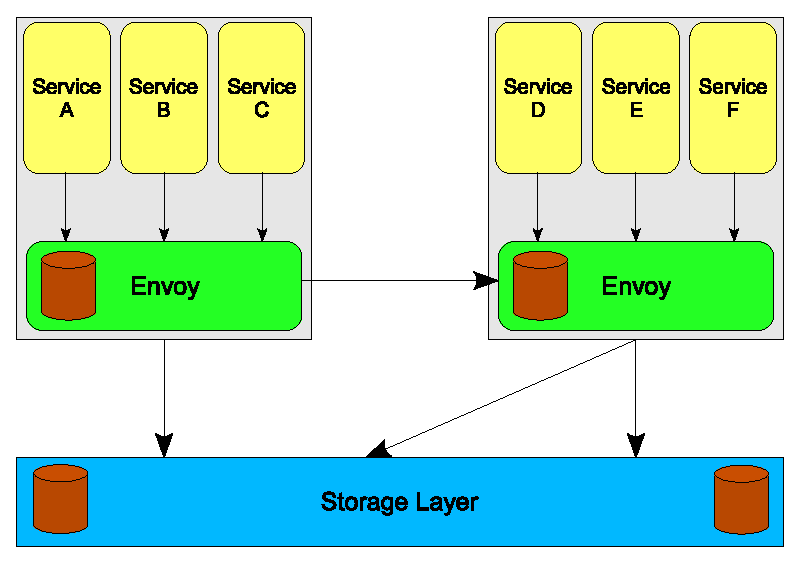
\includegraphics{figures/hops}
\caption{File system requests proceed from service VMs to the local Envoy service. A request from a local territory may be filled by the local in-memory cache, the local disk cache, or by a single network hop to a storage server. A request for a foreign territory adds a single network hop in each case, as the local Envoy acts as the client to a remote Envoy.}
\label{fig:hops}
\end{figure}

\subsubsection{Read operations}\label{sec:data-paths-read}

The best case is a request for hot data in a local territory. In this case, data can be served from the in-memory cache of the local Envoy server. With a fully optimized implementation using Xen or a similar VM environment, this data transfer can occur with a single data copy from the cache to a data page, and that page can then be swapped directly to the client VM via page table manipulation. Since the client's OS does not keep a cached copy, that page can likewise be passed on directly to the client application. While my prototype is not this optimized, the design permits a very lightweight operation involving a single data copy and some metadata manipulation.

Warm data from a local territory follows a similar path, prefaced by retrieving the requested data from the local persistent cache (on disk) into the in-memory cache. With large, cheap commodity disks, the persistent cache can easily hold several operating system images and typical application suites. Typical Linux installations occupy no more than a few gigabytes, and even that includes many supporting files that are rarely used and may never be referenced in common service deployments. If services have forked from standard base images as proposed, it is realistic to assume that the entire operating system and standard applications will be available in the local cache hierarchy for a service being deployed on an active node.

When the local cache fails to deliver, the Envoy service must retrieve requested data from the storage layer. The top half of the storage layer provides a complete object server catalog, so a request can proceed in a single network hop to the node in the storage layer bottom half that hosts the needed object. For simplicity, the persistent cache holds only complete objects, so an entire object must be transfered before the Envoy service can begin fulfilling requests from the local cache. If the object is replicated, the Envoy stripes the transfer across the servers, e.g., if there are three replicas, it streams the first third of the file from the first server, the middle from the second server, and so forth.

Operations in territories outside local control add an extra network hop between the local and remote Envoys for all operations. The data also bypasses the local cache, so locality of reference does nothing to remove this network penalty. It does offer another optimization opportunity (the data, once received from the network, can be passed to the client application without any further copying) but this is minor compensation for a guaranteed latency penalty.

Fortunately, this penalty need not be too great nor too common. The remote Envoy handles the request just as it would one from client local to it, including caching, so referential locality does improve performance from the cold-cache worst case. The target environment is service clusters, too, with high-speed local area networking and unmetered inter-node traffic. Finally, because of the way territories are decided, in a steady state system foreign Envoy requests generally imply some degree of sharing. While relatively uncommon in itself, genuine sharing requires \emph{some} form of synchronous network communication to guarantee consistency, so Envoy's goal of reducing synchronous inter-node to cases of either sharing or infrequent access seems a reasonable one.

\subsubsection{Write operations}

Write operations are less common than reads, but much of the complexity in file system design comes from supporting them. While a good cache satisfies many read requests from memory quickly and with no correctness concerns (provided coherency is maintained in the case of distributed systems), write operations cached in memory raise concerns about durability. If the server acknowledges the write operation as being complete but has only committed it to an in-memory cache, then there is a window of vulnerability before the data is stored to disk and all metadata updated wherein a system crash could lose data that the client expects to be resilient to crashes. In an isolated client, this may be acceptable as the client will simply be forced to restart from the state that was committed to disk and will generally only lose a boundable amount of work. It is particularly problematic for distributed systems and others with external side-effects, however, where other participants may cue subsequent actions on the premise that a write has been successfully and durably committed to disk. The problem is further exacerbated in a commodity hardware environment where failures are routine.

At the other extreme, one can commit all writes to disk before completing the transaction. This makes it clear to the client when a write operation has been consumated, and it is free to either wait for the acknowledgement or proceed asynchronously with explicit knowledge of the risk it is assuming. While this is a simple and appealing model, it ignores two important realities. The first is that the default action for most commodity operating systems is to cache writes and acknowledge them immediately while delaying the disk write. Changing the expected performance characteristics of a basic operation like writing to disk would not provide a commodity-friendly environment as it would severely affect the perforamnce of many standard tools in a negative way. The second is that most files created are short-lived temporary files that are soon deleted \cite{ousterhout}, so synchronously writing them to disk introduces not only unnecessary latency but also unnecessary disk contention.

Several intermediate possibilities exist. Instead of having write requests proceed directly to the storage layer, the local persistent cache could be used as a staging area, with write requests being committed locally and then forwarded to the storage layer after some delay. This would do little to improve performance, however, as synchronous disk access is slower than synchronous network access, so this would not eliminate the slowest link in the event chain. Specialized hardware with involatile memory could also act as a staging area, giving good write performance while retaining durability. The latter approach violates our goal of using widely-available commodity hardware, however, and neither approach is resilient to hardware faults that result in the entire node failing.

Another approach is to only guarantee synchronous durability when explicitly requested by the client, using the equivalent of the Unix \texttt{fsync()} system call. This matches the semantics of local file systems, and thus what most software is written to assume. It is not without faults, however, as the popularity of high-level scripting languages and middleware frameworks (especially for network services, exactly the types of clients service clusters are designed to support) means the connection between application actions and disk operations is often obscured. Requiring low-level controls to get correct behavior is often an acceptable compromise, but it is rarely ideal.

The solution Envoy employs is based on exploiting the cluster environment. While commodity hardware is expected to fail occasionally, simultaneous failure of multiple machines is still relatively rare, provided that the nodes are sufficiently isolated from each other in terms of power and cooling. Since service clusters are intended for professional hosting environments, it is reasonable to assume that hardware faults occur in isolation. With that assumption, durability is less about committing data to disk and more about rudundancy. A write request is considered final when it is in the memory of all of the storage servers that will eventually commit it to disk. If the Envoy server fails, the storage servers are unaffected. If one or more of the storage servers fails before committing the data to disk, the recovery mechanism must restore consistency using the most up-to-date of the replicas. Having storage servers potentially out of sync due to a failed asynchronous write in this scenario is fundamentally no different from having one fail while trying to satisfy a synchronous request. In both cases, the inherent asynchrony of the network means that only the degree of the problem changes.

\section{Operations}

Having examined the high-level architecture of the Envoy file system, I next turn to a more detailed discussion of how specific operations are served. This includes basic file operations and navigation between Envoy instances, the copy-on-write mechanism behind the fork and snapshot operations, coordination of state during territory boundary realignment, security considerations, and the procedure for deleting file system images.

\subsection{Freezing and thawing}

Synchronization at the object level is governed by an important invariant: an object in the system may be referred to by exactly one name in the hierarchical namespace, or it must be read-only. The storage layer makes no attempt to detect or enforce the read-only case, so it is left to the Envoy layer to ensure that this invariant is preserved. To make this straightforward, objects can transition from being writable to read-only, but they can never go back. Note that this refers only to objects in the storage layer, not to the access control of file system objects.

The same invariant makes cache management simple: the Envoy that owns a given territory can cache it without any invalidation concerns, and read-only objects can be safely cached at any number of Envoy nodes without fear of interference. Objects in the cache become invalid only when a territory boundary changes. Objects that are part of ceded territory are not explicitly flushed from the cache; keeping them active helps in two cases: a read-only object may still be referenced by another name in a local territory, and the cache entry (in-memory or on-disk) may still be useful if a file backed by that object is later returned to local control. In the latter case the object must be verified to match the version in the storage layer, but this can be done with a lightweight metadata comparison.

The single mutable/multiple immutable dichotomy in the storage layer is tracked in the Envoy layer through the copy-on-write flag in directory entries. The immutable property is not directly assigned to objects, but instead is imbued by the link from directory to file object. Furthermore, when the immutable object is itself a directory, the property is applied recursively to all of its children, overriding the individual copy-on-write flag in the link to each child. To be regarded as mutable, an object must be reachable by a path from the root of the global namespace to the directory entry linking to the object without traversing any copy-on-write flags that are set.

One immediate consequence of this is that taking a read-only snapshot of a directory and its descendents requires only setting the copy-on-write flag in the link to it, an operation known as \emph{freezing}. Once a directory or file is frozen, the storage layer objects that back the branch rooted at that point are considered immutable. To simplify bookkeeping, this operation is only performed from the root of client images when a snapshot operation is requested. The benefits gained from this restriction and an exception to it are discussed in \prettyref{sec:hard-links}.

The complementary operation is called \emph{thawing}. While the freeze operation works at the root of a subtree and affects it in its entirety, thawing aims to leave as small a footprint as possible; it is always performed with the goal of modifying a particular file. To thaw a file, the owning Envoy starts walking up the line of its ancestors until it finds one that is already thawed. As the root of the namespace cannot be frozen (one can consider it as having a single, implicit link from the Envoy service itself, but there is no mechanism provided to set the copy-on-write flag on this implicit link), this search is guaranteed to succeed. From there the Envoy walks back to the target file, \emph{cloning} intermediate directories as it goes. In addition to making a copy of the directory as its name implies, cloning sets the copy-on-write flag of every directory entry in the copy, effectively transferring the copy-on-write property from the single link leading into the directory to all the links leading out of the directory. The implicit property that each child inherited becomes explicit after being passed down a generation. After thawing each directory for mutability, the parent is updated to reflect both the new object ID and the cleared flag. Eventually the intended target itself (be it file or directory) is cloned, its immediate parent link updated, and the file is fully thawed.

Thawing resembles the procedure for modifying a value in a tree in a functional language. In addition to changing the value itself, the path from that item to the root of the tree must be copied if the item is to be reachable from the root. In the thawing operation, it is only the root of the immutable subtree in which the item resides that must be copied. While the analagous procedure in a functional language copies everything exactly except for the path being changed, the thaw operation must clear the copy-on-write flag as it goes, and thus must push it down from parent link to sibling links at each level in order to preserve the immutable status of the unaffected branches.

\subsection{File and directory operations}

Most basic file and directory operations have a straightforward implementation. The need to cross territory boundaries makes some more complex, however, as they must coordinate with remote Envoys to complete.

\subsubsection{Basic read operations}

The most straightforward operations are \texttt{read} and \texttt{stat}, which read the data and metadata of files, respectively. These requests can be filled using the data paths described in \prettyref{sec:data-paths-read}. The only complication involved is handling the \texttt{atime} attributed, which tracks the last time the data from a file was accessed by a \texttt{read} or \texttt{write} operation. Read operations always proceed through a single Envoy, so this attribute can be tracked accurately: the Envoy can send a message with the timestamp (to ensure that it is consistently applied to all replicas, even if all clocks are not in sync or network latencies between the different storage servers vary) to all replicas in the storage layer which can then update the attribute.

The intended meaning of the \texttt{atime} attribute becomes obscured when applied to frozen files, however. Since attributes are part of the object, akin to \texttt{inodes} in traditional Unix file systems, changing the attribute will affect all files that are backed by that same object. Those instances may be in read-only snapshots of the same file system image, or in common files available in an unrelated file system image. In the former case, the read-only property of the snapshot is broken, and in the latter case the isolation of the two images is compromized. Updating the \texttt{atime} attribute would give an unrelated client using the same prepackaged file system image the ability to losely track file accesses, which could represent a security risk.

Accurately tracking the \texttt{atime} attribute is problematic with frozen files, and if it is only updated on some files (which may change over time as successive snapshots are taken), it is too unreliable to be useful. It also generates network and disk traffic for every read, even those that can be satisfied from the cache. For these reason, the \texttt{atime} attribute is present in Envoy for compatibility, but it effectively mirrors the modified time attribute.

\subsubsection{Reading from directories}

Reading from directories introduces two complications. The first---that successive \texttt{readdir} requests require state that must be transmitted from the client each time or transferred to another Envoy when territories are realigned---is just an implementation issue. The second---that a directory may span multiple territories---requires the cooperation of all affected Envoys. The list of contents for a single directory is considered an atomic unit when drawing territory boundaries, but the files and directories named may be remote. If the client-server protocol used to export the file system to a service only requests names, then the implementation footprint resembles that of file reads. If, as with NFS version~3 and 9p, the response includes attributes as well, additional requests must be forwarded to the respective Envoys for all files that are across a boundary in order to ensure consistent results. These requests are sent directly by the owning Envoy, so if the client is remote, \texttt{readdir} may require the cooperation of three or more Envoys to complete a single request. When gathering file attributes, the Envoy that owns the directory sends requests directly to the file owners, resulting in a star topology with the directory owner as the central node. An additional link from the client's Envoy is necessary if the directory is remotely owned.

Multi-step directory navigation can also create a star pattern of requests, but they always center around the client's local Envoy. Navigating down a series of directories may involve crossing a territory boundary at each step in the extreme case. Because an Envoy confines itself to knowledge of its local territories and their immediate boundaries, it cannot always predict the endpoint Envoy for a navigation. Even if it could, intermediate steps must always be taken to allow permission checking at each level. When a remote territory must be consulted, the client's Envoy forwards all remaining steps in the navigation to the remote owner, which proceeds as far as it can with the navigation. It may return one of three results: if the result is successfully completed, the two Envoys store any state necessary to handle future requests; if the result is a failure, an appropriate error code is returned; if the navigation reaches another territory boundary, the partial result comes back along with a pointer to the Envoy that must be consulted to continue the navigation. The client's Envoy then repeats the procedure with the remaining navigation steps.

Because these operations are all asynchronous, and because the navigated directories may be owned by remote Envoys that are not even neighbors to the client's Envoy, directory navigations may encounter transient failures. Between the time that one remote Envoy returns instructions for forwarding the remainder of a request, the target territory may migrate to a new owner and the request will fail. Because the Envoy that sent the forwarding instructions was an immediate neighbor of the target, its information must have been correct at the time, and careful coordination can ensure that by the time the target bounces the request back with a failure notice, the referrer knows of the change to its immediate neighborhood. The solution is simply to restart the request from the beginning, which will also correct the client's Envoy for the cases of a directory being deleted or renamed.

Generally, having territory boundaries closely aligned with demand benefits everyone, but if multi-step directory navigations are frequent, their performance will be hurt by frequent boundaries. Caching navigation results can be done safely with a few precautions. First note that a navigation that succeeds one time and fails another implies one of three things: one of the steps was deleted or renamed, permissions changed somewhere, or a different user requested the navigation. Envoy caches navigation results keyed by the path traversed and the user that requested it. With the assumption that directory renames and permission changes are uncommon (particularly across boundaries determined by locality of reference---I expect these changes to be most common in a region being actively modified by a single player, not in higher-level directories whose descendents are in active use by different clients), Envoys broadcast notification of such changes down the hierarchy when they occur, invalidating cached navigation results.

Attributes at the endpoint of the navigation are always confirmed directly with the owner, as are all of the final steps that occurred on territory owned by that same Envoy. With a hot cache, multi-step directory navigations are satisfied from the cache of the client's Envoy and a single step to the Envoy hosting the target of the navigation.

\subsubsection{Basic write operations}
thaw + mtime
\subsubsection{Deleting files}
\subsubsection{Renaming files}
walk invalidations
\subsubsection{Hard links}\label{sec:hard-links}
dead object in storage layer? special log file/hidden directory catalog?

\subsection{Forks and snapshots}

A few additional rules simplify management. The root of the namespace is always writable, as are all administrative directories, i.e., those that are not descendents of a directory called \current or one of its numbered snapshots. Snapshots are always immutable

\subsection{Lease migration}
\subsection{Security}
\subsection{Deleting snapshots}

\section{Dynamic lease management}

What we really want is a dedicated guy running around setting up little servers near the interested clients and rearranging them as traffic stabalizes. A healthy dose of laziness may even be an asset---keep it simple and avoid thrashing.

\section{Recovery}

\section{Summary}